\chapter{Mouvements dans un champ uniforme}

\textit{La mécanique du point matériel permet de décrire le mouvement d’un projectile dans le champ de pesanteur terrestre, ainsi que celui d’une particule chargée dans un champ électrique uniforme. Ces deux situations, fondamentales en physique, illustrent l’application du principe fondamental de la dynamique et des lois de conservation. Ce chapitre établit les équations horaires, les caractéristiques des trajectoires (parabole, portée, flèche) et aborde les aspects énergétiques.}

% ===================================================================
\section{Projectile dans le champ de pesanteur uniforme}

\subsection{Champ de pesanteur et modèle du projectile}

On considère un objet de masse $m$, lancé dans le champ de pesanteur terrestre, supposé uniforme : $\vect{g} = -g\,\vect{k}$ (axe $Oz$ vertical ascendant). On néglige les frottements de l’air et la poussée d’Archimède. Le système est le projectile, étudié dans le référentiel terrestre galiléen.

\begin{definition}[Projectile]
Un projectile est un corps lancé dans l’espace, soumis uniquement à son poids $\vect{P}=m\vect{g}$. On néglige toute autre force (frottement, portance).
\end{definition}

\begin{loi}[Principe fondamental de la dynamique]
Dans le référentiel terrestre galiléen, la somme des forces extérieures appliquées au projectile est égale à sa masse multipliée par son accélération :
\[
\sum \vect{F}_{\text{ext}} = m\,\vect{a} \quad\Longrightarrow\quad m\vect{g} = m\,\vect{a}
\]
d’où $\vect{a} = \vect{g}$.
\end{loi}

\subsection{Équations horaires}

On choisit un repère cartésien $(O,\vect{i},\vect{j},\vect{k})$ avec $O$ au point de lancement, $\vect{i}$ horizontal, $\vect{j}$ horizontal perpendiculaire (mouvement plan), $\vect{k}$ vertical ascendant. Les conditions initiales sont :
\[
\vect{v}_0 = v_0\cos\alpha\,\vect{i} + v_0\sin\alpha\,\vect{k}, \qquad \vect{r}_0 = \vect{0}.
\]

Par intégration successive de $\vect{a} = -g\,\vect{k}$, on obtient :
\begin{align*}
\vect{v}(t) &= v_0\cos\alpha\,\vect{i} + \bigl(v_0\sin\alpha - gt\bigr)\,\vect{k},\\
\vect{r}(t) &= \bigl(v_0\cos\alpha\,t\bigr)\,\vect{i} + \bigl(v_0\sin\alpha\,t - \frac12 g t^2\bigr)\,\vect{k}.
\end{align*}

\begin{propriete}[Équations horaires paramétriques]
\[
\begin{cases}
x(t) = v_0\cos\alpha\; t,\\[2pt]
y(t) = 0,\\[2pt]
z(t) = v_0\sin\alpha\; t - \dfrac12 g t^2.
\end{cases}
\]
Le mouvement est plan dans le plan $(Oxz)$.
\end{propriete}

\subsection{Équation de la trajectoire}

En éliminant le temps $t = \dfrac{x}{v_0\cos\alpha}$, on obtient :
\[
z(x) = x\tan\alpha - \frac{g}{2v_0^2\cos^2\alpha}\,x^2.
\]

\begin{loi}[Trajectoire parabolique]
La trajectoire d’un projectile dans un champ de pesanteur uniforme, en l’absence de frottements, est une parabole d’axe vertical.
\end{loi}

\begin{illus}
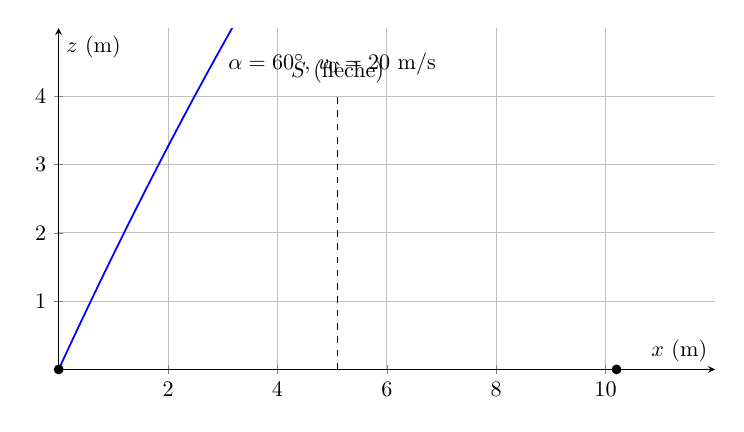
\begin{tikzpicture}[scale=0.8]
\begin{axis}[
    axis lines=middle,
    xlabel=$x$ (m), ylabel=$z$ (m),
    xmin=0, xmax=12, ymin=0, ymax=5,
    xtick={2,4,6,8,10}, ytick={1,2,3,4},
    grid=both,
    width=12cm, height=7cm,
    samples=100,
    domain=0:10.2,
    ]
    \addplot[thick,blue] {x*tan(60) - 9.8*x^2/(2*20^2*cos(60)^2)};
    \addplot[only marks,mark=*] coordinates {(0,0) (10.2,0)};
    \node[above] at (axis cs:5,4.2) {$\alpha=60^\circ$, $v_0=20$~m/s};
    \node[below] at (axis cs:0,0) {$O$};
    \node[below] at (axis cs:10.2,0) {$P$};
    \draw[dashed] (axis cs:5.1,0) -- (axis cs:5.1,4.08);
    \node[above] at (axis cs:5.1,4.08) {$S$ (flèche)};
\end{axis}
\end{tikzpicture}
\fig{Figure 3.1 — Trajectoire parabolique d’un projectile : portée $OP$ et flèche $z_S$.}
\end{illus}

\subsection{Portée et flèche}

\begin{definition}[Portée]
La portée $P$ est la distance horizontale parcourue par le projectile lorsqu’il retombe à la même altitude qu’au départ ($z=0$).
\end{definition}

En résolvant $z(x)=0$ (hors $x=0$) :
\[
x_P = \frac{v_0^2\sin(2\alpha)}{g}.
\]
La portée est maximale pour $\alpha=45^\circ$ : $x_{P,\max} = \dfrac{v_0^2}{g}$.

\begin{definition}[Flèche]
La flèche $z_S$ est l’altitude maximale atteinte par le projectile. Elle correspond à $v_z=0$, soit $t_S = \dfrac{v_0\sin\alpha}{g}$, d’où :
\[
z_S = \frac{v_0^2\sin^2\alpha}{2g}.
\]
\end{definition}

\begin{remarque}
La flèche est indépendante de la masse du projectile (dans le modèle sans frottement).
\end{remarque}

\subsection{Aspects énergétiques}

Le poids étant une force conservative, l’énergie mécanique se conserve :
\[
E_m = \frac12 m v^2 + mgz = \text{constante} = \frac12 m v_0^2.
\]
En un point quelconque de la trajectoire :
\[
v^2 = v_0^2 - 2gz.
\]

\begin{aretenir}
Pour un projectile sans frottement, l’énergie mécanique est constante. La vitesse est maximale au départ et à l’arrivée ($z=0$), minimale au sommet ($z=z_S$).
\end{aretenir}

% ===================================================================
\section{Particule chargée dans un champ électrique uniforme}

\subsection{Force électrique et accélération}

Une particule de charge $q$ et de masse $m$, placée dans un champ électrique uniforme $\vect{E}$, subit la force électrostatique :
\[
\vect{F}_e = q\,\vect{E}.
\]

\begin{loi}[Principe fondamental de la dynamique]
\[
q\,\vect{E} = m\,\vect{a} \quad\Longrightarrow\quad \vect{a} = \frac{q}{m}\,\vect{E}.
\]
L’accélération est constante et colinéaire au champ $\vect{E}$.
\end{loi}

\subsection{Mouvement entre les armatures d’un condensateur plan}

On considère un condensateur plan dont les armatures sont distantes de $d$, soumises à une tension $U$. Le champ électrique est uniforme :
\[
E = \frac{U}{d}, \qquad \vect{E} = -E\,\vect{k} \quad (\text{de l’armature positive vers la négative}).
\]

Une particule de charge $q>0$ pénètre en $O$ avec une vitesse initiale $\vect{v}_0 = v_0\,\vect{i}$ (horizontale). Les équations du mouvement s’obtiennent par intégration de $\vect{a} = -\dfrac{qE}{m}\,\vect{k}$ :
\begin{align*}
\vect{v}(t) &= v_0\,\vect{i} - \frac{qE}{m}t\,\vect{k},\\
\vect{r}(t) &= v_0 t\,\vect{i} - \frac12\frac{qE}{m}t^2\,\vect{k}.
\end{align*}

\begin{propriete}[Déviation électrostatique]
La trajectoire est une parabole dans le plan $(Oxz)$. La déviation verticale à la sortie du condensateur (longueur $L$) est :
\[
z(L) = -\frac{qE L^2}{2m v_0^2}.
\]
\end{propriete}

\begin{illus}
\begin{circuitikz}[scale=0.9, transform shape]
\draw (0,0) to[short,o-] (1,0) to[V=$U$] (1,-3) to[short,-o] (0,-3);
\draw (2,0) -- (5,0) node[above] {$+$};
\draw (2,-3) -- (5,-3) node[below] {$-$};
\draw[->,thick] (2.5,-1.5) -- (3.5,-1.5) node[midway,above] {$\vect{v}_0$};
\draw[->,thick] (3.5,-1.5) -- (4.5,-2.5) node[midway,right] {$\vect{v}$};
\draw[dashed] (2.5,-1.5) parabola (4.5,-2.5);
\node at (2.5,-1.5) {$\bullet$};
\node[above] at (2.5,-1.5) {$O$};
\node at (4.5,-2.5) {$\bullet$};
\node[below] at (4.5,-2.5) {$S$};
\draw[->,thick] (5.5,-1.5) -- (6.5,-1.5) node[right] {$\vect{E}$};
\end{circuitikz}
\fig{Figure 3.2 — Déviation d’une particule chargée entre les armatures d’un condensateur plan.}
\end{illus}

\subsection{Application à l’oscilloscope cathodique}

Dans un oscilloscope, un faisceau d’électrons est dévié par des plaques de déviation verticale (et horizontale). La déviation $z$ est proportionnelle à la tension appliquée $U$ :
\[
z = \frac{q L^2}{2m d v_0^2}\,U.
\]
Cela permet de visualiser des signaux électriques.

\begin{remarque}
La sensibilité verticale $S_v = \dfrac{z}{U}$ s’exprime en \si{\centi\metre\per\volt}.
\end{remarque}

\subsection{Aspects énergétiques}

Le champ électrique uniforme dérive d’un potentiel $V$ : $\vect{E} = -\vect{\nabla}V$. La force électrique est conservative. L’énergie potentielle électrostatique est $E_p = qV$. L’énergie mécanique se conserve :
\[
\frac12 m v^2 + qV = \text{constante}.
\]

\begin{aretenir}
La variation d’énergie cinétique entre deux points $A$ et $B$ est égale au travail de la force électrique :
\[
\Delta E_c = q(V_A - V_B) = qU_{AB}.
\]
\end{aretenir}

% ===================================================================
\section{L’essentiel à retenir}

\begin{synthese}
\paragraph{Projectile dans le champ de pesanteur}
\begin{itemize}
\item Accélération : $\vect{a} = \vect{g}$ (constante).
\item Équations horaires : $x = v_0\cos\alpha\,t$, $z = v_0\sin\alpha\,t - \frac12 g t^2$.
\item Trajectoire : $z(x) = x\tan\alpha - \dfrac{g}{2v_0^2\cos^2\alpha}\,x^2$ (parabole).
\item Portée : $P = \dfrac{v_0^2\sin(2\alpha)}{g}$ ; maximale pour $\alpha=45^\circ$.
\item Flèche : $z_S = \dfrac{v_0^2\sin^2\alpha}{2g}$.
\item Conservation de l’énergie mécanique : $\frac12 m v^2 + mgz = \frac12 m v_0^2$.
\end{itemize}

\paragraph{Particule chargée dans un champ $\vect{E}$ uniforme}
\begin{itemize}
\item Force : $\vect{F}_e = q\vect{E}$ ; accélération : $\vect{a} = \dfrac{q}{m}\vect{E}$.
\item Mouvement parabolique si $\vect{v}_0 \perp \vect{E}$.
\item Déviation : $z = \dfrac{qE L^2}{2m v_0^2}$ (condensateur plan).
\item Conservation de l’énergie : $\frac12 m v^2 + qV = \text{cte}$.
\end{itemize}

\paragraph{Unités et pièges}
\begin{itemize}
\item $g$ en \si{\metre\per\second\squared}, $v_0$ en \si{\metre\per\second}, $U$ en \si{\volt}, $E$ en \si{\volt\per\metre}.
\item Ne pas confondre $E$ (champ électrique) et $E$ (énergie).
\item La portée est nulle pour $\alpha=0^\circ$ ou $90^\circ$ (tir vertical).
\item Le signe de $q$ détermine le sens de la déviation.
\end{itemize}
\end{synthese}

% ===================================================================
\section{Méthodes \& savoir-faire}

\methode{Établir les équations horaires d’un projectile}
\begin{enumerate}
\item Définir le repère et les conditions initiales.
\item Appliquer le PFD : $\vect{a} = \vect{g}$.
\item Intégrer pour obtenir $\vect{v}(t)$, puis $\vect{r}(t)$.
\item Écrire les équations paramétriques.
\end{enumerate}
\begin{exemple}
Un joueur de football frappe un ballon avec $v_0=\SI{15}{\metre\per\second}$ sous un angle $\alpha=30^\circ$. Établir les équations horaires.
\emph{Solution :} $x=15\cos30^\circ\,t$, $z=15\sin30^\circ\,t - 4,9 t^2$.
\end{exemple}

\methode{Calculer la portée et la flèche}
\begin{enumerate}
\item Pour la portée : résoudre $z(x)=0$ (hors $x=0$).
\item Pour la flèche : annuler $v_z(t)$ pour trouver $t_S$, puis $z(t_S)$.
\end{enumerate}
\begin{exemple}
Avec $v_0=\SI{20}{\metre\per\second}$, $\alpha=45^\circ$, calculer $P$ et $z_S$.
\emph{Solution :} $P = \frac{20^2\sin90^\circ}{9,8} \approx \SI{40,8}{\metre}$ ; $z_S = \frac{20^2\sin^2 45^\circ}{2\times9,8} \approx \SI{10,2}{\metre}$.
\end{exemple}

\methode{Étudier la déviation d’une particule chargée}
\begin{enumerate}
\item Déterminer $\vect{E}$ à partir de $U$ et $d$.
\item Appliquer le PFD : $\vect{a} = \frac{q}{m}\vect{E}$.
\item Intégrer avec $\vect{v}_0$ donné.
\item Calculer la déviation à la sortie du condensateur.
\end{enumerate}
\begin{exemple}
Un électron ($q=-e$, $m=\SI{9.11e-31}{\kilogram}$) pénètre à $v_0=\SI{2e7}{\metre\per\second}$ entre deux plaques distantes de $d=\SI{2}{\centi\metre}$ avec $U=\SI{100}{\volt}$. Quelle est sa déviation après $L=\SI{5}{\centi\metre}$ ?
\emph{Solution :} $E=U/d=\SI{5000}{\volt\per\metre}$ ; $z = -\frac{(-e)E L^2}{2m v_0^2} = \frac{1.6e-19\times5000\times(0.05)^2}{2\times9.11e-31\times(2e7)^2} \approx \SI{2.75}{\centi\metre}$ (vers le haut).
\end{exemple}

\methode{Appliquer la conservation de l’énergie}
\begin{enumerate}
\item Identifier les forces conservatives.
\item Écrire $E_m = E_c + E_p = \text{cte}$.
\item Relier les vitesses aux positions.
\end{enumerate}
\begin{exemple}
Un projectile lancé de $z=0$ avec $v_0=\SI{10}{\metre\per\second}$ atteint une hauteur $h$. Calculer $h$.
\emph{Solution :} $\frac12 m v_0^2 = mgh$ $\Rightarrow$ $h = \frac{v_0^2}{2g} \approx \SI{5,1}{\metre}$.
\end{exemple}

\methode{Utiliser les symétries}
\begin{itemize}
\item La trajectoire est symétrique par rapport à la verticale passant par le sommet.
\item La durée de montée égale la durée de descente.
\end{itemize}
\begin{exemple}
Un projectile met \SI{2}{\second} pour atteindre son sommet. Quelle est sa vitesse initiale verticale ?
\emph{Solution :} $v_{0z}=g t_S = 9,8\times2 = \SI{19,6}{\metre\per\second}$.
\end{exemple}

\methode{Relier déviation et tension dans un oscilloscope}
\begin{exemple}
Un oscilloscope a une sensibilité verticale de \SI{2}{\centi\metre\per\volt}. Quelle tension produit une déviation de \SI{4}{\centi\metre} ?
\emph{Solution :} $U = \frac{z}{S_v} = \frac{4}{2} = \SI{2}{\volt}$.
\end{exemple}

\methode{Choisir le bon angle pour une portée maximale}
\begin{exemple}
Quel angle donne la plus grande portée pour $v_0$ fixé ?
\emph{Solution :} $\alpha=45^\circ$ car $\sin(2\alpha)$ est maximal.
\end{exemple}

\methode{Étudier un tir vertical}
\begin{exemple}
Un projectile est lancé verticalement vers le haut avec $v_0=\SI{15}{\metre\per\second}$. Quelle hauteur atteint-il ?
\emph{Solution :} $h = \frac{15^2}{2\times9,8} \approx \SI{11,5}{\metre}$.
\end{exemple}

\methode{Analyser un mouvement dans un champ $\vect{E}$ avec vitesse initiale oblique}
\begin{exemple}
Une particule $q>0$ pénètre avec $\vect{v}_0$ faisant un angle $\theta$ avec l’horizontale dans un champ $\vect{E}$ vertical. Décrire le mouvement.
\emph{Solution :} Mouvement parabolique dans le plan contenant $\vect{v}_0$ et $\vect{E}$ ; équations similaires au projectile avec $g$ remplacé par $qE/m$.
\end{exemple}

% ===================================================================
\section{Exercices d’application}

\rubrique{Projectile dans le champ de pesanteur}

\exo{}\diff{1} Un joueur de basket lance le ballon avec une vitesse $v_0=\SI{8}{\metre\per\second}$ sous un angle $\alpha=60^\circ$. Calculer la portée et la flèche.

\exo{}\diff{2} Un projectile est lancé du sol avec $v_0=\SI{30}{\metre\per\second}$ et $\alpha=30^\circ$. Déterminer :
\begin{enumerate}
\item Les équations horaires.
\item La durée totale du vol.
\item La vitesse au sommet.
\end{enumerate}

\exo{}\diff{2} Un canon tire un obus avec $v_0=\SI{100}{\metre\per\second}$ sous un angle $\alpha=45^\circ$. À quelle distance tombe-t-il ? Quelle est sa hauteur maximale ?

\exo{}\diff{3} Un projectile est lancé d’une hauteur $h=\SI{10}{\metre}$ avec $v_0=\SI{15}{\metre\per\second}$ horizontalement. Établir l’équation de la trajectoire et calculer la distance horizontale parcourue avant de toucher le sol.

\rubrique{Particule chargée dans un champ $\vect{E}$ uniforme}

\exo{}\diff{1} Un proton ($q=+e$, $m=\SI{1.67e-27}{\kilogram}$) est accéléré par une tension $U=\SI{500}{\volt}$. Quelle est sa vitesse acquise ?

\exo{}\diff{2} Un électron pénètre à $v_0=\SI{1e7}{\metre\per\second}$ entre deux plaques parallèles distantes de $d=\SI{1}{\centi\metre}$ avec $U=\SI{200}{\volt}$. Calculer la déviation après $L=\SI{4}{\centi\metre}$.

\exo{}\diff{2} Une particule $\alpha$ ($q=+2e$, $m=\SI{6.64e-27}{\kilogram}$) traverse un condensateur de longueur $L=\SI{10}{\centi\metre}$ avec $v_0=\SI{5e6}{\metre\per\second}$. La tension est $U=\SI{1000}{\volt}$, $d=\SI{2}{\centi\metre}$. Quelle est sa déviation ?

\exo{}\diff{3} Dans un oscilloscope, un électron est dévié de \SI{3}{\centi\metre} par une tension $U=\SI{1.5}{\volt}$. Quelle est la sensibilité verticale ?

\rubrique{Aspects énergétiques}

\exo{}\diff{1} Un projectile de masse $m=\SI{0.5}{\kilogram}$ est lancé avec $v_0=\SI{20}{\metre\per\second}$. Quelle est son énergie cinétique initiale ? Quelle hauteur maximale peut-il atteindre ?

\exo{}\diff{2} Un électron est accéléré par une tension $U=\SI{1000}{\volt}$. Calculer sa vitesse finale.

\exo{}\diff{2} Un projectile de masse $m=\SI{2}{\kilogram}$ est lancé verticalement avec $v_0=\SI{15}{\metre\per\second}$. En utilisant la conservation de l’énergie, déterminer la hauteur atteinte.

\exo{}\diff{3} Une particule chargée ($q=+3.2e-19$~C, $m=\SI{2e-26}{\kilogram}$) est lancée dans un champ $\vect{E}$ uniforme de \SI{5000}{\volt\per\metre} avec $v_0=\SI{1e4}{\metre\per\second}$ perpendiculaire au champ. Calculer la variation d’énergie cinétique après avoir parcouru \SI{5}{\centi\metre} dans la direction du champ.

\rubrique{Synthèse}

\exo{}\diff{3} Un projectile est lancé du sol avec $v_0=\SI{25}{\metre\per\second}$ sous un angle $\alpha$. On observe que sa portée est de \SI{50}{\metre}. Déterminer $\alpha$ (deux solutions). Calculer la flèche correspondante.

\exo{}\diff{3} Un électron pénètre dans un condensateur plan avec $v_0=\SI{2e7}{\metre\per\second}$ parallèlement aux armatures. La tension est $U=\SI{300}{\volt}$, $d=\SI{1.5}{\centi\metre}$, $L=\SI{6}{\centi\metre}$. Déterminer la déviation à la sortie et la vitesse de l’électron à cet instant.

% ===================================================================
\section{Exercices d’entraînement}

\rubrique{Projectile dans le champ de pesanteur}

\exo{}\diff{1} Un ballon est lancé avec $v_0=\SI{12}{\metre\per\second}$ sous $\alpha=40^\circ$. Calculer la portée.

\exo{}\diff{2} Un projectile est lancé du sol avec $v_0=\SI{40}{\metre\per\second}$ et $\alpha=60^\circ$. Déterminer la hauteur maximale et la durée du vol.

\exo{}\diff{2} Un joueur de football tire un penalty : le ballon part à $v_0=\SI{20}{\metre\per\second}$ sous $\alpha=30^\circ$. La cage est à \SI{11}{\metre}. Le ballon passe-t-il au-dessus de la barre transversale (hauteur \SI{2.44}{\metre}) ?

\exo{}\diff{3} Un projectile est lancé d’une falaise de hauteur $H=\SI{50}{\metre}$ avec $v_0=\SI{30}{\metre\per\second}$ horizontalement. Calculer la distance horizontale parcourue avant l’impact.

\exo{}\diff{3} Un obus est tiré avec $v_0=\SI{200}{\metre\per\second}$ sous $\alpha=30^\circ$. Quelle est la portée ? Quelle est la vitesse à l’impact ?

\exo{}\diff{2} Un projectile lancé avec $v_0=\SI{15}{\metre\per\second}$ atteint une hauteur maximale de \SI{5}{\metre}. Quel est l’angle de lancement ?

\exo{}\diff{3} Un athlète lance un poids avec $v_0=\SI{10}{\metre\per\second}$ sous $\alpha=45^\circ$ d’une hauteur de \SI{2}{\metre}. Quelle est la portée ?

\exo{}\diff{2} Deux projectiles sont lancés avec la même vitesse $v_0$ mais des angles $\alpha$ et $90^\circ-\alpha$. Montrer qu’ils ont la même portée.

\rubrique{Particule chargée dans un champ $\vect{E}$ uniforme}

\exo{}\diff{1} Un électron est accéléré par une tension $U=\SI{500}{\volt}$. Calculer sa vitesse.

\exo{}\diff{2} Un proton pénètre dans un condensateur avec $v_0=\SI{3e6}{\metre\per\second}$ perpendiculairement au champ. $U=\SI{400}{\volt}$, $d=\SI{2}{\centi\metre}$, $L=\SI{8}{\centi\metre}$. Calculer la déviation.

\exo{}\diff{3} Une particule $\alpha$ est déviée de \SI{2}{\centi\metre} dans un condensateur de $L=\SI{10}{\centi\metre}$, $d=\SI{1}{\centi\metre}$, $U=\SI{500}{\volt}$. Quelle est sa vitesse initiale ?

\exo{}\diff{2} Un oscilloscope a une sensibilité de \SI{1.5}{\centi\metre\per\volt}. Quelle tension produit une déviation de \SI{6}{\centi\metre} ?

\exo{}\diff{3} Un électron est émis avec une vitesse nulle d’une plaque négative vers une plaque positive distante de $d=\SI{5}{\centi\metre}$ avec $U=\SI{2000}{\volt}$. Calculer sa vitesse à l’arrivée.

\exo{}\diff{2} Deux particules de masses différentes mais de même charge sont accélérées par la même tension. Laquelle a la plus grande vitesse ?

\rubrique{Aspects énergétiques}

\exo{}\diff{1} Un projectile de masse $m=\SI{1}{\kilogram}$ est lancé avec $v_0=\SI{10}{\metre\per\second}$. Quelle est son énergie mécanique ?

\exo{}\diff{2} Un électron est accéléré par $U=\SI{2000}{\volt}$. Calculer son énergie cinétique en \si{\joule} et en \si{\electronvolt}.

\exo{}\diff{3} Une particule chargée ($q=+e$) est lancée dans un champ $\vect{E}$ uniforme de \SI{1000}{\volt\per\metre} avec $v_0=\SI{2e5}{\metre\per\second}$ perpendiculaire au champ. Après quelle distance dans la direction du champ sa vitesse a-t-elle doublé ?

\exo{}\diff{2} Un projectile de masse $m=\SI{0.2}{\kilogram}$ est lancé verticalement avec $v_0=\SI{12}{\metre\per\second}$. Utiliser la conservation de l’énergie pour trouver la hauteur maximale.

\rubrique{Synthèse}

\exo{}\diff{3} Un projectile est lancé du sol avec $v_0=\SI{50}{\metre\per\second}$ sous un angle $\alpha$. La portée est de \SI{200}{\metre}. Déterminer $\alpha$ et la flèche.

\exo{}\diff{3} Un électron pénètre dans un condensateur plan avec $v_0=\SI{1.5e7}{\metre\per\second}$ parallèlement aux armatures. $U=\SI{250}{\volt}$, $d=\SI{1.2}{\centi\metre}$, $L=\SI{5}{\centi\metre}$. Déterminer la déviation et la vitesse à la sortie.

\exo{}\diff{3} Un projectile est lancé d’une hauteur $h=\SI{20}{\metre}$ avec $v_0=\SI{25}{\metre\per\second}$ sous $\alpha=30^\circ$. Calculer la portée et la vitesse à l’impact.

\exo{}\diff{3} Une particule de charge $q$ et de masse $m$ est lancée dans un champ $\vect{E}$ uniforme avec $\vect{v}_0$ faisant un angle $\theta$ avec $\vect{E}$. Décrire qualitativement le mouvement.

% ===================================================================
\section{Sujets type Baccalauréat}

\sujetbac[Projectile dans le champ de pesanteur]
Un projectile de masse $m=\SI{0.1}{\kilogram}$ est lancé du sol avec une vitesse initiale $v_0=\SI{20}{\metre\per\second}$ sous un angle $\alpha=30^\circ$ par rapport à l’horizontale. On néglige les frottements.
\begin{enumerate}
\item Établir les équations horaires du mouvement.
\item Déterminer l’équation de la trajectoire.
\item Calculer la portée et la flèche.
\item Quelle est l’énergie mécanique du projectile ? En déduire sa vitesse au sommet.
\item Si le projectile était lancé avec le même $v_0$ mais sous un angle $\alpha=45^\circ$, quelle serait la nouvelle portée ?
\end{enumerate}

\sujetbac[Déviation d’un électron dans un oscilloscope]
Un oscilloscope cathodique utilise un faisceau d’électrons accélérés par une tension $U_a=\SI{2000}{\volt}$ entre la cathode et l’anode. Les électrons pénètrent ensuite entre deux plaques de déviation verticale de longueur $L=\SI{4}{\centi\metre}$, distantes de $d=\SI{1.5}{\centi\metre}$, soumises à une tension $U_d$.
\begin{enumerate}
\item Calculer la vitesse $v_0$ des électrons à la sortie de l’accélérateur.
\item Établir l’expression de la déviation $z$ à la sortie des plaques en fonction de $U_d$, $L$, $d$, $v_0$ et des constantes.
\item Calculer $z$ pour $U_d=\SI{100}{\volt}$.
\item Quelle est la sensibilité verticale de l’oscilloscope ?
\item Si on double $U_a$, comment la sensibilité est-elle modifiée ?
\end{enumerate}

\sujetbac[Étude énergétique d’un projectile et d’une particule chargée]
\begin{enumerate}
\item Un projectile de masse $m=\SI{0.5}{\kilogram}$ est lancé verticalement avec $v_0=\SI{15}{\metre\per\second}$. En utilisant la conservation de l’énergie, déterminer la hauteur maximale atteinte.
\item Un électron est accéléré par une tension $U=\SI{1000}{\volt}$. Calculer sa vitesse finale.
\item Comparer les deux situations : quelles sont les similitudes et les différences du point de vue énergétique ?
\end{enumerate}

% ===================================================================
\section{Corrigés}

\corrige{de l’exercice 1}
\textbf{Projectile — portée et flèche.}
\begin{itemize}
\item $P = \dfrac{v_0^2\sin(2\alpha)}{g} = \dfrac{8^2\sin120^\circ}{9,8} \approx \dfrac{64\times0,866}{9,8} \approx \SI{5,66}{\metre}$.
\item $z_S = \dfrac{v_0^2\sin^2\alpha}{2g} = \dfrac{64\times(\sin60^\circ)^2}{19,6} = \dfrac{64\times0,75}{19,6} \approx \SI{2,45}{\metre}$.
\end{itemize}

\corrige{de l’exercice 2}
\textbf{Projectile — équations horaires, durée, vitesse au sommet.}
\begin{enumerate}
\item $x = 30\cos30^\circ\,t = 25,98\,t$ ; $z = 30\sin30^\circ\,t - 4,9 t^2 = 15t - 4,9t^2$.
\item Durée totale : $z=0 \Rightarrow t(15-4,9t)=0 \Rightarrow t=0$ ou $t=15/4,9 \approx \SI{3,06}{\second}$.
\item Au sommet, $v_z=0$ donc $v = v_x = 30\cos30^\circ \approx \SI{25,98}{\metre\per\second}$.
\end{enumerate}

\corrige{de l’exercice 3}
\textbf{Canon — portée et flèche.}
\begin{itemize}
\item $P = \dfrac{100^2\sin90^\circ}{9,8} = \dfrac{10000}{9,8} \approx \SI{1020,4}{\metre}$.
\item $z_S = \dfrac{100^2\sin^2 45^\circ}{2\times9,8} = \dfrac{10000\times0,5}{19,6} \approx \SI{255,1}{\metre}$.
\end{itemize}

\corrige{de l’exercice 4}
\textbf{Projectile lancé horizontalement d’une hauteur.}
\begin{itemize}
\item Équations : $x = 15t$, $z = 10 - 4,9t^2$.
\item Trajectoire : $z = 10 - \dfrac{4,9}{225}x^2$.
\item Impact : $z=0 \Rightarrow t = \sqrt{10/4,9} \approx \SI{1,43}{\second}$ ; $x = 15\times1,43 \approx \SI{21,45}{\metre}$.
\end{itemize}

\corrige{de l’exercice 5}
\textbf{Proton accéléré.}
$v = \sqrt{\dfrac{2qU}{m}} = \sqrt{\dfrac{2\times1,6e-19\times500}{1,67e-27}} \approx \sqrt{9,58e10} \approx \SI{3,09e5}{\metre\per\second}$.

\corrige{de l’exercice 6}
\textbf{Électron dans un condensateur.}
$E = U/d = 200/0,01 = \SI{20000}{\volt\per\metre}$.
$z = \dfrac{qE L^2}{2m v_0^2} = \dfrac{1,6e-19\times20000\times(0,04)^2}{2\times9,11e-31\times(1e7)^2} \approx \dfrac{1,6e-19\times20000\times0,0016}{2\times9,11e-31\times1e14} = \dfrac{5,12e-18}{1,822e-16} \approx \SI{0,0281}{\metre} = \SI{2,81}{\centi\metre}$.

\corrige{de l’exercice 7}
\textbf{Particule $\alpha$ dans un condensateur.}
$E = 1000/0,02 = \SI{50000}{\volt\per\metre}$.
$z = \dfrac{2\times1,6e-19\times50000\times(0,1)^2}{2\times6,64e-27\times(5e6)^2} = \dfrac{1,6e-19\times50000\times0,01}{6,64e-27\times2,5e13} = \dfrac{8e-17}{1,66e-13} \approx \SI{4,82e-4}{\metre} = \SI{0,482}{\milli\metre}$.

\corrige{de l’exercice 8}
\textbf{Sensibilité verticale.}
$S_v = z/U = 3/1,5 = \SI{2}{\centi\metre\per\volt}$.

\corrige{de l’exercice 9}
\textbf{Énergie cinétique et hauteur.}
$E_c = \frac12 m v_0^2 = 0,5\times0,5\times400 = \SI{100}{\joule}$.
$h_{\max} = \dfrac{v_0^2}{2g} = \dfrac{400}{19,6} \approx \SI{20,4}{\metre}$.

\corrige{de l’exercice 10}
\textbf{Électron accéléré.}
$v = \sqrt{\dfrac{2eU}{m}} = \sqrt{\dfrac{2\times1,6e-19\times1000}{9,11e-31}} \approx \sqrt{3,51e14} \approx \SI{1,87e7}{\metre\per\second}$.

\corrige{de l’exercice 11}
\textbf{Hauteur par conservation de l’énergie.}
$\frac12 m v_0^2 = mgh \Rightarrow h = \dfrac{v_0^2}{2g} = \dfrac{225}{19,6} \approx \SI{11,5}{\metre}$.

\corrige{de l’exercice 12}
\textbf{Variation d’énergie cinétique.}
$E = \SI{5000}{\volt\per\metre}$, $d = \SI{0,05}{\metre}$ dans la direction du champ.
$W = qEd = 3,2e-19\times5000\times0,05 = \SI{8e-17}{\joule}$.
$\Delta E_c = W = \SI{8e-17}{\joule}$.

\corrige{de l’exercice 13}
\textbf{Angle pour une portée donnée.}
$P = \dfrac{v_0^2\sin(2\alpha)}{g} \Rightarrow \sin(2\alpha) = \dfrac{Pg}{v_0^2} = \dfrac{50\times9,8}{625} = 0,784$.
$2\alpha = \arcsin(0,784) \approx 51,6^\circ$ ou $128,4^\circ$, donc $\alpha \approx 25,8^\circ$ ou $64,2^\circ$.
Flèche pour $\alpha=25,8^\circ$ : $z_S = \dfrac{625\times\sin^2 25,8^\circ}{19,6} \approx \dfrac{625\times0,189}{19,6} \approx \SI{6,03}{\metre}$.
Pour $\alpha=64,2^\circ$ : $z_S = \dfrac{625\times\sin^2 64,2^\circ}{19,6} \approx \dfrac{625\times0,811}{19,6} \approx \SI{25,9}{\metre}$.

\corrige{de l’exercice 14}
\textbf{Électron dans un condensateur — déviation et vitesse.}
$E = 300/0,015 = \SI{20000}{\volt\per\metre}$.
$z = \dfrac{eE L^2}{2m v_0^2} = \dfrac{1,6e-19\times20000\times(0,06)^2}{2\times9,11e-31\times(2e7)^2} = \dfrac{1,6e-19\times20000\times0,0036}{2\times9,11e-31\times4e14} = \dfrac{1,152e-17}{7,288e-16} \approx \SI{0,0158}{\metre} = \SI{1,58}{\centi\metre}$.
$v_x = v_0 = \SI{2e7}{\metre\per\second}$ ; $v_z = -\dfrac{eE}{m}t = -\dfrac{eE L}{m v_0} = -\dfrac{1,6e-19\times20000\times0,06}{9,11e-31\times2e7} \approx -\dfrac{1,92e-16}{1,822e-23} \approx -\SI{1,05e7}{\metre\per\second}$.
$v = \sqrt{v_x^2+v_z^2} = \sqrt{4e14+1,1025e14} \approx \sqrt{5,1025e14} \approx \SI{2,26e7}{\metre\per\second}$.

\corrige{du sujet 1}
\textbf{Projectile — Bac.}
\begin{enumerate}
\item $x = 20\cos30^\circ\,t = 17,32t$ ; $z = 20\sin30^\circ\,t - 4,9t^2 = 10t - 4,9t^2$.
\item $z = x\tan30^\circ - \dfrac{9,8}{2\times20^2\cos^2 30^\circ}x^2 = 0,577x - \dfrac{9,8}{600}x^2 = 0,577x - 0,01633x^2$.
\item $P = \dfrac{20^2\sin60^\circ}{9,8} = \dfrac{400\times0,866}{9,8} \approx \SI{35,35}{\metre}$ ; $z_S = \dfrac{400\times0,25}{19,6} \approx \SI{5,10}{\metre}$.
\item $E_m = \frac12 m v_0^2 = 0,5\times0,1\times400 = \SI{20}{\joule}$. Au sommet, $v = v_x = 17,32$~m/s, $E_c = 0,5\times0,1\times300 = \SI{15}{\joule}$, $E_p = mgz_S = 0,1\times9,8\times5,1 \approx \SI{5}{\joule}$.
\item $P_{45^\circ} = \dfrac{400\times\sin90^\circ}{9,8} \approx \SI{40,82}{\metre}$.
\end{enumerate}

\corrige{du sujet 2}
\textbf{Oscilloscope — Bac.}
\begin{enumerate}
\item $v_0 = \sqrt{\dfrac{2eU_a}{m}} = \sqrt{\dfrac{2\times1,6e-19\times2000}{9,11e-31}} \approx \sqrt{7,03e14} \approx \SI{2,65e7}{\metre\per\second}$.
\item $z = \dfrac{eU_d L^2}{2m d v_0^2}$.
\item $z = \dfrac{1,6e-19\times100\times(0,04)^2}{2\times9,11e-31\times0,015\times(2,65e7)^2} = \dfrac{1,6e-19\times100\times0,0016}{2\times9,11e-31\times0,015\times7,0225e14} = \dfrac{2,56e-20}{1,918e-17} \approx \SI{1,33e-3}{\metre} = \SI{1,33}{\milli\metre}$.
\item $S_v = z/U_d = 1,33e-3/100 = \SI{1,33e-5}{\metre\per\volt} = \SI{1,33e-3}{\centi\metre\per\volt}$.
\item Si $U_a$ double, $v_0$ est multipliée par $\sqrt{2}$, donc $z$ est divisée par 2, et $S_v$ aussi.
\end{enumerate}

\corrige{du sujet 3}
\textbf{Étude énergétique — Bac.}
\begin{enumerate}
\item $\frac12 m v_0^2 = mgh \Rightarrow h = \dfrac{v_0^2}{2g} = \dfrac{225}{19,6} \approx \SI{11,5}{\metre}$.
\item $v = \sqrt{\dfrac{2eU}{m}} = \sqrt{\dfrac{2\times1,6e-19\times1000}{9,11e-31}} \approx \SI{1,87e7}{\metre\per\second}$.
\item Similitudes : dans les deux cas, l’énergie potentielle (gravitationnelle ou électrostatique) se transforme en énergie cinétique et vice versa. Différences : la force est conservative dans les deux cas, mais l’énergie potentielle gravitationnelle dépend de $g$ et de la hauteur, tandis que l’énergie potentielle électrostatique dépend de la charge et de la tension.
\end{enumerate}

\endinput